\documentclass{llncs}
%\pagestyle{plain}

\usepackage[cmex10]{amsmath}
\usepackage{amssymb}
\usepackage{array}
\usepackage{bm}
\usepackage{graphicx}
\usepackage{epstopdf}
\usepackage[hang]{subfigure}
\usepackage{import}
\usepackage{booktabs}
\usepackage{tabularx}
\usepackage{pdfpages}
\usepackage{epstopdf}
\graphicspath{{figures/}}
\usepackage{wrapfig}
\usepackage[export]{adjustbox}
\usepackage[font=scriptsize]{caption}
\usepackage{mwe}


%\usepackage[colorlinks=true,linkcolor=blue,citecolor=blue,urlcolor=black]{hyperref}
\usepackage{algorithm, algpseudocode}
%\algsetup{linenosize=\scriptsize}

% Commenting functionality
%\usepackage{todonotes}
%\reversemarginpar

\newcommand{\brs}[1]{\left[{#1}\right]} %square bracets
\newcommand{\brr}[1]{{\left({#1}\right)}} %round bracets
\newcommand{\brf}[1]{\left\lbrace{#1}\right\rbrace} %figure bracets
\newcommand{\brabs}[1]{\left\vert{#1}\right\vert} %absolute bracets
\newcommand{\norm}[2]{\left\|{#1}\right\|_{#2}} %norm_*

\newcommand{\I}[1]{I\!\left[{#1}\right]} %Robustness criterion I[*]
\newcommand{\Iq}[1]{I_q\!\left[{#1}\right]} %Robustness criterion I_q[*]
\newcommand{\Ic}[1]{I_c\!\left[{#1}\right]} %Robustness criterion I_c[*]

\newcommand{\vx}{\mathbf{x}} % vector x
\newcommand{\vy}{\mathbf{y}} % vector y
\newcommand{\vX}{\mathbf{X}} % vector X
\newcommand{\vf}{\mathbf{f}} % vector f
\newcommand{\vz}{\mathbf{z}} % vector z
\newcommand{\vZ}{\mathbf{Z}} % vector Z
\newcommand{\vw}{\mathbf{w}} % vector w
\newcommand{\vd}{\mathbf{d}} % vector d
\newcommand{\vp}{\mathbf{p}} % vector p
\newcommand{\vP}{\mathbf{P}} % vector P
\newcommand{\vu}{\mathbf{u}} % vector u
\newcommand{\vU}{\mathbf{U}} % vector U
\newcommand{\DSet}{\mathcal{D}} % Set D
\newcommand{\NSet}{\mathcal{N}} % Set N
\newcommand{\XSet}{\mathcal{X}} % set X
\newcommand{\ZSet}{\mathcal{Z}} % set Z
\newcommand{\SSet}{\mathcal{S}} % set S
\newcommand{\ISet}{\mathcal{I}} % set I
\newcommand{\Pref}{\mathcal{P}} % Preferences set P

\DeclareMathOperator*{\argmin}{\arg\!\min}
\DeclareMathOperator*{\argmax}{\arg\!\max}


\begin{document}
\title{sParEGO -- A Hybrid Optimization Algorithm for Expensive Uncertain Multi-Objective Optimization Problems}
\author{Jo\~{a}o A. Duro\inst{1} \and Robin C. Purshouse\inst{1} \and Shaul Salomon\inst{1,2} \and Daniel C. Oara\inst{1} \and Visakan Kadirkamanathan\inst{1} \and Peter J. Fleming\inst{1}}
\institute{University of Sheffield, UK \email{\{j.a.duro,r.purshouse\}@sheffield.ac.uk}
\and ORT Braude College of Engineering, Israel, \email{shaulsal@braude.ac.il}}

\maketitle

\begin{abstract}
Evaluations of candidate solutions to real-world problems are often expensive to compute, are characterised by uncertainties arising from multiple sources, and involve simultaneous consideration of multiple conflicting objectives. Here, the task of an optimizer is to find a set of solutions that offer alternative robust trade-offs between objectives, where robustness comprises some user-defined measure of the ability of a solution to retain high performance in the presence of uncertainties. Typically, understanding the robustness of a solution requires multiple evaluations of performance under different uncertain conditions -- but such an approach is infeasible for expensive problems with a limited evaluation budget. To overcome this issue, a new hybrid optimization algorithm for expensive uncertain multi-objective optimization problems is proposed. The algorithm -- sParEGO -- uses a novel uncertainty quantification approach to assess the robustness of a candidate design without having to rely on expensive sampling techniques. Hypotheses on the relative performance of the algorithm compared to an existing method for deterministic problems are tested using two benchmark problems, and provide preliminary indication that sParEGO is an effective technique for identifying robust trade-off surfaces.
\keywords{Expensive optimization, surrogate-based optimization, robust optimization, multi-objective optimization}
\end{abstract}

\section{Introduction}

The ability of simulations to predict the performance of a candidate design is constantly increasing. While some simulations can produce high-fidelity outputs relatively quickly, a typical mesh-based simulation can run for several hours, and even days. Even if a design team has access to supercomputing resources, the extensive run-time still implies that perhaps only a few hundred candidate designs can be explored using high-fidelity modelling resources. Unfortunately, conventional multi-objective optimization algorithms implemented in commercial packages typically require tens of thousands of function evaluations to converge on a high quality solution~\cite{Zhou2011Multiobjective}. Therefore, the search for a promising design using expensive evaluation functions on a limited computational budget poses a great challenge.

To exacerbate this problem, optimizing for a robust solution is itself a computationally demanding task. In order to gain confidence over the robustness of a solution to uncertainties, the statistical properties of the expected solution's performance must be quantified. In a world where the complexity of the high-fidelity models essentially produces a black-box mapping of inputs to outputs, such statistical properties would typically be found through repeated evaluation of the same solution using those high-fidelity models. However, repeatedly sampling a single candidate design is computationally expensive.

To address the above, we propose a framework for expensive uncertain multi-objective optimization problems. The key aims are to: (i) exploit expensive, black-box evaluation function for a candidate design; (ii) account for multiple sources of uncertainty, such as fidelity of evaluation functions and manufacturing tolerances; and (iii) provide an understanding of the risk and opportunity trade-offs between candidate designs with respect to a given robustness metric. To achieve this the framework leverages ParEGO~\cite{Knowles2006ParEGO}, an algorithm for multi-objective optimization, which has been demonstrated to provide good results for optimization runs limited to a small number of function evaluations. ParEGO itself is a multi-objective extension to Jones et al.'s~\cite{Jones1998Efficient} seminal efficient global optimization (EGO) algorithm for single-objective problems. The main limitation of ParEGO is that it has not been designed to handle problems featuring uncertainty (although
there is some evidence that it can perform favourably in noisy environments~\cite{knowles2009noisy}). Therefore a fundamental part of the framework is how ParEGO can be extended to consider evaluation functions as samples of random variates. We refer to this new algorithm as \emph{stochastic ParEGO} or \emph{sParEGO}. 

In the remainder of this paper, first the robustness metric used is described in Section~\ref{sec:robustness_metric}, and the proposed framework is presented in Section~\ref{sec:framework}. The test suite used is defined in Section~\ref{sec:test_suite}, while the experimental settings and obtained results are in Section~\ref{sec:results}. The paper concludes with Section~\ref{sec:conclusion}.

\section{Threshold-based robustness metric}\label{sec:robustness_metric}

A general single-objective robust optimisation problem can be formulated as:
\begin{align}
\min_{\vx\in\Omega} S=\vf\brr{\vx,\vU}.
\label{eq:rev:robust}
\end{align}
Here, $\vU$ is a vector of random variables that includes all the uncertainties associated with the optimisation problem. These uncertainties may be an outcome of manufacturing tolerances, a noisy environment, evaluation inaccuracies etc. A single scenario of the variate $\vU$ is denoted as $\vu$. Since uncertainties are involved, the scalar objective $S$ is also a random variate, where every scenario of the uncertainties, $\vu$, is associated with an objective value $s$.

In a robust optimisation scheme, the random objective value is replaced with a robustness criterion, denoted by the indicator $\I{S}$. Several criteria are commonly used in the literature, which can be broadly categorised into three main approaches:
\begin{enumerate}
\item \textbf{Worst-Case Scenario.} The worst objective vector, considering a bounded domain in the neighbourhood of the nominal values of the uncertain variables.
\item \textbf{Aggregated Value.} An integral measure of robustness that amalgamates the possible values of the uncertain variables (e.g. mean value or variance).
\item \textbf{Threshold Probability.} The probability for the objective function to be better than a defined threshold.
\end{enumerate}

In this framework the third approach, suggested by Beyer and Sendhof~\cite{Beyer2007}, is used. A threshold $q$ is considered as a satisfying performance for the objective value $s$. When $s$ is uncertain, denoted by the random variable $S$, the probability for $S$ to satisfy the threshold level can be seen as a confidence level $c$. For a minimization problem this can be written as:
\begin{align}
c\brr{S,q}=\text{Pr}\brr{S<q}.
\label{eq:confidence}
\end{align}
A robustness indicator used in this paper is based on minimization of the threshold $q$ for a pre-defined confidence level $c$, meaning that the confidence in the resulting performance can be specified (say by a decision-maker).

A stochastic unconstrained multi-objective optimization problem (MOP), which is the focus of this study, can be formulated as:
\begin{align}
\label{eq:mop}
	\min_{\vx\in\Omega} \vZ=\vf\brr{\vx, \vU}.
\end{align}
where $\vx$ is a vector of $n_x$ decision variables in a feasible domain $\Omega$, $\vZ$ is a multivariate random vector of $n_z$ performance criteria and $\vf$ is a set of functions mapping from decision-space to objective-space. Due to uncertainties over the problem parameters or the mapping functions themselves, every evaluation of the same decision vector may result in a different realisation of the objective vector $\vz$.

\section{The Framework of the sParEGO Algorithm}\label{sec:framework}

\subsection{General Framework}

sParEGO is a surrogate-based multi-objective optimization algorithm for dealing with stochastic multi-objective optimization problems (MOPs). The algorithm shares many similarities with ParEGO including the ability to approximate expensive MOPs over a realistically small number of function evaluations. The main idea is that the uncertain distribution in objective space of every candidate solution is not quantified through uncertainty quantification methods (e.g. Monte Carlo sampling). Instead, every solution is evaluated once, and the distribution is approximated based on the performance of nearby solutions. A pseudo-code of sParEGO is presented in Algorithm~\ref{alg:sParEGO}. Its stages are explained in detail in the remainder of this section.

\begin{algorithm}
\scriptsize
\caption{\textsc{sParEGO} Pseudo-code}
\label{alg:sParEGO}
\begin{algorithmic}[1]
	\Statex \textbf{Parameters:} initial set size $n_\text{init}$, robustness criterion $I$, evaluation functions $\vf$,
	\Statex \hspace{20mm} neighbourhood distance $\delta$, number of reference direction vectors $n_d$
	\State $\DSet \leftarrow$ a set of all reference direction vectors
	\State $\XSet \leftarrow$ initialise a set with neighbourhoods of solutions \Comment{Section~\ref{subsec:initialisation}}
	\State $\ZSet \leftarrow \vf\brr{\XSet}$ \Comment{evaluate the initial set}
	\While{stopping criteria not satisfied}
		\State Shuffle the set $\DSet$
		\ForAll{$\vd\in\DSet$}
			\ForAll{$\vx^i\in\XSet$}
				\State update neighbourhood $\NSet^i$ \Comment{Section~\ref{subsec:Uncertainty quantification}}
			\EndFor
			\State update ideal and nadir vectors
			\State $\SSet \leftarrow$ calculate scalar fitness value of all solutions
			\State $\ISet \leftarrow \emptyset$
			\ForAll{$\vx^i\in\XSet$}
				\State approximate the distribution of $S^i$ \Comment{Section~\ref{subsec:Uncertainty quantification}}
				\State calculate robustness indicator $\I{S^i}$ \Comment{Section~\ref{subsec:robustness indicators}}
				\State $\ISet \leftarrow \ISet \cup \I{S^i}$
			\EndFor
			\State $model \leftarrow$ fit a Surrogate model to the indicator values $\ISet$ \Comment{Section~\ref{subsec:Kriging}}
			\State $\vx^\text{new} \leftarrow$ maximize the expected improvement based on $model$
			\State $\vx^\text{pert} \leftarrow$ add a neighbour to $\vx^\text{new}$ \Comment{Section~\ref{subsec:Kriging}} 
			\State $\XSet \leftarrow \XSet \cup \brf{\vx^\text{new}, \vx^\text{pert}}$
			\State $\ZSet \leftarrow \ZSet \cup \brf{\vf\brr{\vx^\text{new}}, \vf\brr{\vx^\text{pert}}}$ \Comment{evaluate the new solutions}
		\EndFor
	\EndWhile
\end{algorithmic}
\end{algorithm}

\subsection{Parameters}\label{subsec:Parameters}
\begin{itemize}
\item $\delta$ -- Neighbourhood distance. Maximum Euclidean distance between solutions, in normalised decision space (i.e. between 0 and 1), to be considered as neighbours. Default value is $0.1 \sqrt{n_x}$.
\item $n_\text{init}$ -- Size of initial population.
\item $n_\text{indp}$ -- Portion of solutions in the initial population that are independently generated. Must be smaller or equal to $n_\text{init}/2$.
\item $\delta_\text{pert}$ -- Maximum distance between newly generated solutions. Default value is $\delta / 2$.
\item $c$ -- Desired level of confidence in the performance of the solutions.
\item $n_\text{max}$ -- Maximum number of solutions to construct the Surrogate model.
\end{itemize}

\subsection{Initialisation}\label{subsec:initialisation}

To provide good initial coverage of potential designs, a space filling design (Latin hypercube) is used for the initial set. However, the algorithm requires all solutions to reside within a distance of $\delta$ from other solutions (at least one).
To accomplish this, only $n_\text{indp} \leq n_\text{init}/2$ solutions are generated by Latin hypercube sampling. The rest of the solutions are generated as follows:
\begin{enumerate}
\item For every existing solution, another solution is randomly generated within a hypersphere with a radius of $\delta_\text{pert}$.
\item The rest of the solutions are generated by randomly selecting an existing solution and creating a nearby solution within a distance of $\delta_\text{pert}$.
\end{enumerate}
The first stage enforces that every solution has at least one neighbour.
The second stage seeds the initial population with neighbourhoods of different sizes.


\subsection{Uncertainty quantification}\label{subsec:Uncertainty quantification}

The most important difference between sParEGO and ParEGO is that the former assumes that the outcome of an evaluation function is a realization of a random variate. Therefore, the scalarised function value cannot be used directly to construct the surrogate model, and a utility indicator value is used instead. For every direction vector, the surrogate model is constructed to search for a design that will optimize a given robustness indicator (described later in Section~\ref{subsec:robustness indicators}). The guiding principle is to avoid having to repeatedly sample every candidate design to assess its statistical properties in objective-space. Instead, these properties (specifically, measures of central tendency and dispersion) are approximated from the available information of other candidate design evaluations.

\subsubsection{Approximation of the central tendency}

The stochasticity of the problem might originate from a variety of sources, including variations in decision-space. For this type of uncertainty, two designs with similar nominal values can be identical when realised. Therefore, the performance of a candidate design should be calculated from the performance of neighbouring designs as well. A distance\footnote{Distance is measured in decision-space by the Euclidean norm.} in normalised\footnote{The decision vectors are normalised between 0 and 1.} decision space $\delta$ is defined, such that two solutions $\vx^i$ and $\vx^j$ are considered as neighbours if:
\begin{align}
	\norm{\vx^i-\vx^j}{2}\leq\delta.
\end{align}
For a solution $\vx^i$, the statistical properties of the scalar fitness are approximated from the neighbouring solutions as follows:
First, the neighbourhood $\NSet^i$ of the solution is defined\footnote{Note that according to~\eqref{eq:neighbourhood}, $\vx^i$ is included in the neighbourhood $\NSet^i$.}:
\begin{align}
	\label{eq:neighbourhood}
	\NSet^i=\brf{\vx^j\in \XSet \,\vert \,\norm{\vx^i-\vx^j}{2}\leq\delta}.
\end{align}
Next, the approximated mean function value, $\mu_s$, is derived from the neighbourhood.
Members that are closer to $\vx^i$ are given a larger weight, denoted as $v$ in Equation~\eqref{eq:neighbourhood weights}, in approximating its properties.
Since the weight of most solutions in the neighbourhood is smaller than 1, the overall "neighbourhood size" $N^i$ is smaller than $\brabs{\NSet^i}$:
\begin{align}
	\label{eq:neighbourhood weights}
	v^j &= \frac{\delta-\norm{\vx^i-\vx^j}{2}}{\delta}, \quad  \forall \vx^j\in\NSet^i,\\
	\label{eq:neighbourhood size}
	N^i &= \sum_{\vx^j\in\NSet^i} v^j,\\
	\label{eq:neighbourhood mean}
	\mu^i_s &= \left. \sum_{\vx^j\in\NSet^i} v^j s^j \middle/ N^i \right. .
\end{align}

\subsubsection{Approximation of the dispersion}

Once the expected mean is known, the expected value for the variance is calculated:
\begin{align}
	\label{eq:neighbourhood variance}	\sigma^{2,i}_s = \left. \sum_{\vx^j\in\NSet^i} v^j \brr{s^j - \mu^i_s}^2 \middle/ N^i \right. .
\end{align}


\begin{figure}
\centering
\subfigure[Estimation of the mean value and the variance from the neighbourhood]{
	\def\svgwidth{0.44\textwidth}
	\import{figures/}{indicator_estimation_1.pdf_tex}
	\label{subfig:indicator_estimation_1}
}
\hspace{1mm}
\subfigure[Assuming a normal distribution for $S$ according to $\mu_s$ and $\sigma_s$. The shaded area represents a confidence of $80\%$.]{
	\def\svgwidth{0.44\textwidth}
	\import{figures/}{indicator_estimation_2.pdf_tex}
	\label{subfig:indicator_estimation_2}
}
\caption{Approximation of the statistical properties, and estimation of robustness indicator $\Ic{\bullet}$.}
\label{fig:indicator_estimation}
\end{figure}

\subsection{Estimating the robustness indicator value}\label{subsec:robustness indicators}

Once the mean and variance of the scalar fitness function have been estimated for every solution in the set, the random variable $S\brr{\vx}$ is assumed to follow a normal distribution. Given a desired confidence level $c$, the robustness indicator $\Ic{S}$ can be calculated. An example for $\Ic{S}$ is given in Figure~\ref{subfig:indicator_estimation_2} where $\Ic{S}$ value corresponds to the 80$^{th}$ percentile of the normal distribution. This implies that the obtained $\Ic{S}$ value depends on the chosen confidence. Following this, the indicator value $\Ic{S}$ is considered as the solution's fitness at the current iteration.

\subsection{Fitting a Surrogate Model to the Fitness}\label{subsec:Kriging}

Now that every solution is associated with a scalar fitness value based on the robust indicator, the algorithm proceeds in a similar fashion to EGO and ParEGO~\cite{Jones1998Efficient,knowles2005multiobjective}. A surrogate model is fitted to the fitness values, and the expected improvement function is constructed from the model. This requires the variance in the expected improvement function ($\hat{\sigma}^2$) to be estimated. For this we use the density of the solutions in decision-space by knowing that the variance has an inverse correlation to the density of the solutions. A suitable way to estimate the density at a given point $\vx$ is to use a non-parametric statistical approach, and in this case we use a kernel density model given by:
\begin{equation}
 p(\vx) = \frac{1}{N} \sum^{N}_{n=1} \frac{1}{(2\pi h^2)^{D/2}}   \exp\left\{-\frac{\| \vx-\vx_n \|^2}{2h^2}\right\},
\end{equation}
where $N$ is the number of points, $D$ is the number of dimensions, and $h$ is the bandwidth. We let the bandwidth be equal to 1/100$^{th}$ of the mean span of all points, that is:
\begin{equation}
 h = \frac{1}{100N}\sum_{n=1}^{N} (\max(\vx_n) - \min(\vx_n)).
\end{equation}

Based on experimental results we have observed that the kernel density model can be very sensitive to any changes in the density, thus we have used a smoothing function (in this case the $\arctan$ function), and the estimated variance at input $\vx$ is given by:
\begin{equation}
 \hat{\sigma}^2(\vx) = \left( \frac{1}{\pi/2} \arctan \left(\frac{1}{p(\vx)}\right) \right)^2.
\end{equation}

Above a certain size (approximately 50 solutions), the surrogate model becomes prohibitively expensive to construct. When the number of evaluated solutions exceed this size, a subset of size $n_\text{max}$ is is chosen according to Algorithm~\ref{alg:filtration}.

\begin{algorithm}
\caption{Choosing a Subset to Construct the Surrogate Model}
\label{alg:filtration}
\begin{algorithmic}[1]
	\Require population set $\XSet$, subset size $n_\text{max}$, current direction vector $\vd$
	\Ensure a subset $\XSet'$ of size $n_\text{max}$
	\State $\XSet' \leftarrow n_\text{max}/2$ solutions from $\XSet$ with the best indicator value
	\State $\XSet'' \leftarrow \XSet \setminus \XSet'$
	\ForAll{$\vx \in \XSet''$}
		\State $\hat{\vz}\brr{\vx} \leftarrow$ normalise $\vz\brr{\vx}$ and project it on the $k-1$ simplex
		\State $\Delta\brr{\vx, \vd} \leftarrow \norm{\hat{\vz}\brr{\vx} - \vd}{2}$
	\EndFor
	\State $\XSet' \leftarrow \XSet' \cup n_\text{max}/2$ solutions from $\XSet''$ with the smallest $\Delta$ distance
\end{algorithmic}
\end{algorithm}

The next step is to search for the solution that maximises the expected improvement. For this task, any off-the-shelf single-objective optimizer can be used, and we have chosen ACROMUSE~\cite{Ginley2011}. Once a solution $\vx^\text{new}$ that maximizes the expected improvement is identified, it is added to the population together with a neighbouring solution $\vx^\text{pert}$, generated in a similar fashion to the initial solutions described in Section~\ref{subsec:initialisation}.

\section{Test Suite}\label{sec:test_suite}

The test suite used in this paper consists of two variants of WFG4~\cite{bib:wfg_2006}. Both problems have two objectives and five decision variables. For the first problem, namely P1, we have modified WFG4 to increase the density and the number of local optima in the periphery of the global optimum. This simulates the effect that stochasticity can have when approaching the Pareto-optimal Front (PF). The second problem, namely P2, is characterised by having a more smooth landscape with no local minima surrounding the global optimum, and stochasticity is added by the toolkit from~\cite{Salomon2016Toolkit}.

The modification applied to WFG4 is as follows. The original formulation of WFG4 applies a transformation to each input parameter ($y$) given by:
\begin{equation}
\begin{aligned}
 \text{s\_multi}(y,A,B,C) &= \left(1+\cos(r_2) +B (r_1)^2  
 \right)/(B+2),\\
 r_1 &= |y-C| / (\lfloor C-y \rfloor +C ),\\
 r_2 &= (4A+2)\pi ( 0.5 - 0.5r_1 ),
 \label{eq:wfg4_t1}
\end{aligned}
 \end{equation}
where $A$ controls the number of minima, $B$ controls the magnitude of the ``hill sizes'' of the multi-modality, and $C$ is the value for which $y$ is mapped to zero. We propose a modification to Equation~\ref{eq:wfg4_t1} as follows:
\begin{equation}
\begin{aligned}
 \text{s\_multi}^*(y,A,B,C,D,E) &= \left( 1+\cos(r_2 r_3) +B|r_1|^E  \right)/(B+2),\\
 r_3 &= (1-|r_1|)^{2D},
\end{aligned}
 \label{eq:wfg4_t1_mod}
\end{equation}
where $D$ controls the density of the hills around the optimum, and $E$ specifies the polynomial order of the base curve. The effect of these parameters is shown in Figure~\ref{fig:transformation_function}, in that:
\begin{enumerate}
 \item the number of minima increases up-to $2A+1=11$ for $A=5$, which includes the global optimum at $C=0.45$, as shown in Figure~\ref{fig:transformation_function-a};
 \item density of hills around the optimum increases with an increase in $D$ as shown in Figure~\ref{fig:transformation_function-b}; and
 \item the proximity of local minima from the value zero decreases with an increase in $E$ as shown in Figure~\ref{fig:transformation_function-c}.
\end{enumerate}

\begin{figure}
\centering
\subfigure[Modality]{
 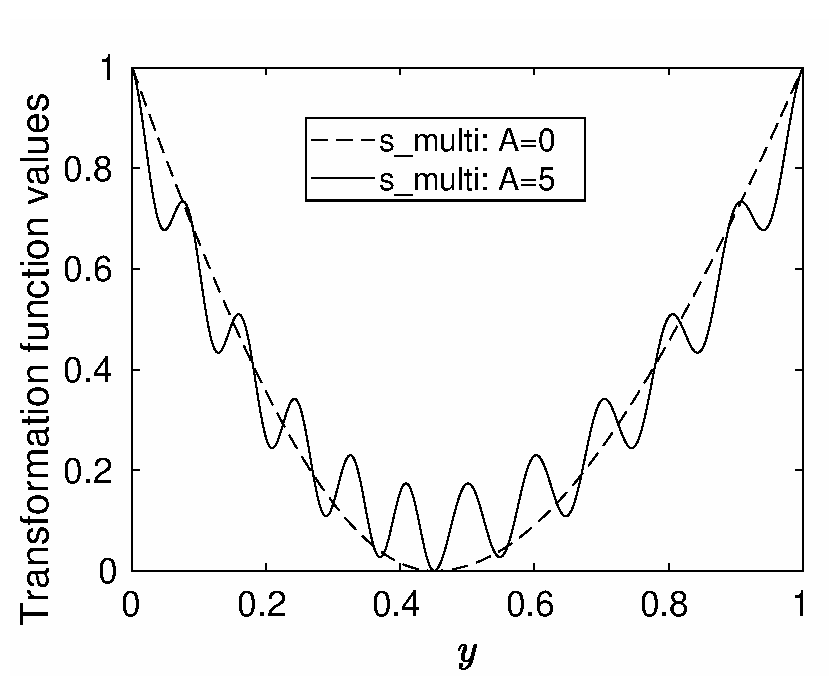
\includegraphics[width=0.31\textwidth]{figures/TestProblemsModality_a.eps}
 \label{fig:transformation_function-a}
}
\subfigure[Density]{
 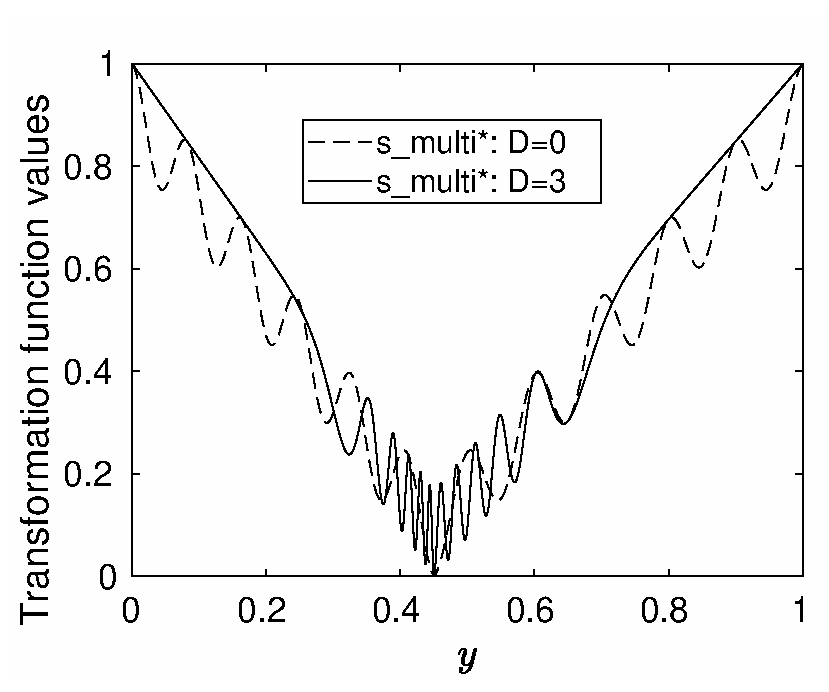
\includegraphics[width=0.31\textwidth]{figures/TestProblemsModality_b.eps}
 \label{fig:transformation_function-b}
}
\subfigure[Proximity to zero]{
 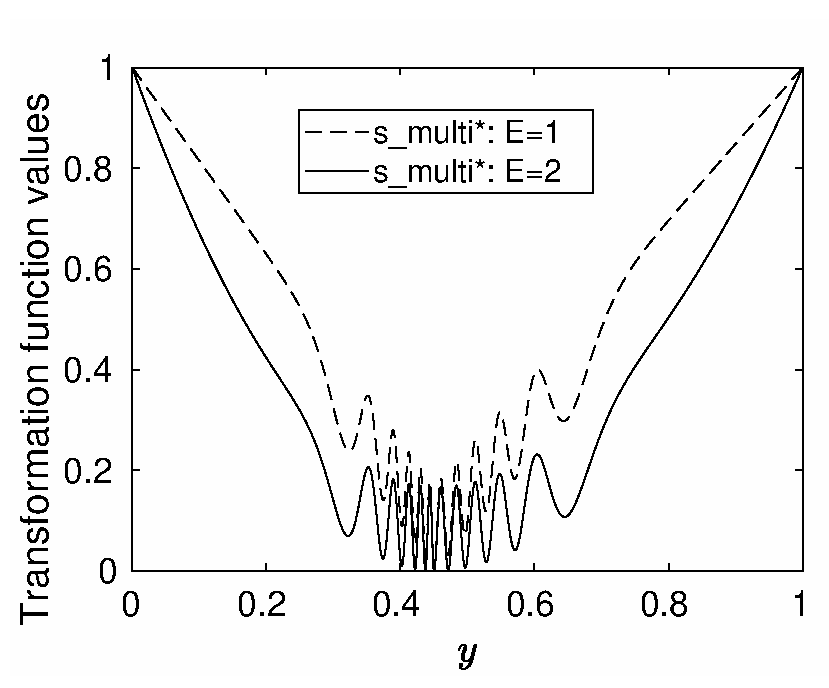
\includegraphics[width=0.31\textwidth]{figures/TestProblemsModality_c.eps}
 \label{fig:transformation_function-c}
}
 \caption{Transformation function in WFG4 as a function of the input parameter ($y$). The parameters $B=10$ and $C=0.45$ are kept fixed for all cases. For (b) $A=5$, $E=1$ and for (c) $A=5$, $D=3$.}
 \label{fig:transformation_function}
\end{figure}

The toolkit from~\cite{Salomon2016Toolkit} is used here to transform the objective vectors of WFG4 into random vectors. The parameters have been chosen to ensure that uncertainty increases towards more optimal regions, and perturbation is applied to the objective vector in only one direction (known as the radial component), hence the perturbation radius is set to zero. The radial component uses a uniform distribution with a lower bound ($l_b$) which depends on the position of the normalised objective vector with respect to the reference vector $(2/3,1.0)$. Another parameter of the distribution is locality ($l$), and its value is determined by an increasing function that uses the remoteness of the objective vector raised to the power of 0.4. The upper bound is given by $ub=1-l(1-lb)$. 

Following the above, we have chosen $C=0.45$ for all test instances. The remaining parameters are: $A=5$, $B=10$, $D=3$, and $E=1$ for P1; and $A=0$, $B=8$, $D=0$, and $E=2$ for P2. The obtained PF for P1 and P2 are shown in Figures~\ref{fig:reference_sets_p1_PF} and~\ref{fig:reference_sets_p2_PF}, respectively. The performance set for P1 and P2 have been obtained by fixing the values of the last three decision variables to 2.1, 2.8 and 3.5, respectively, as suggested in the WFG toolkit paper~\cite{bib:wfg_2006}. The values of the first two decision variables have been determined by NSGA-II~\cite{deb2002fast}\footnote{NSGA-II has been run for 10000 generations with the following settings: the distribution index of SBX-crossover and polynomial mutation set to 15 and 20, respectively; and probability of crossover and mutation set to 90\% and 10\%, respectively.} with a population size of 300 solutions, since crowding distance is able to provide a reasonable diverse set across the PF. The robust set for P2 has been obtained by replacing the uniform distribution of the radial component by the 90th percentile of the same distribution (assuming a confidence level of 90\%). NSGA-II is used again with the same settings to determine the values of the decision variables that better satisfy the chosen robustness indicator.

Notably for P2 as shown in Figure~\ref{fig:reference_sets_p2_PS}, the decision vectors that are Pareto-optimal with respect to the performance criterion are different from the decision vectors that are Pareto-optimal with respect to the robustness criterion. The implication is that an optimal solution set cannot satisfy the performance and robustness criterion simultaneously. Therefore, we use the terms performance PF and robust PF to refer to objective vectors that are Pareto-optimal with respect to either the performance or robustness criterion.

\begin{figure}
\centering
\subfigure[P1: PF]{
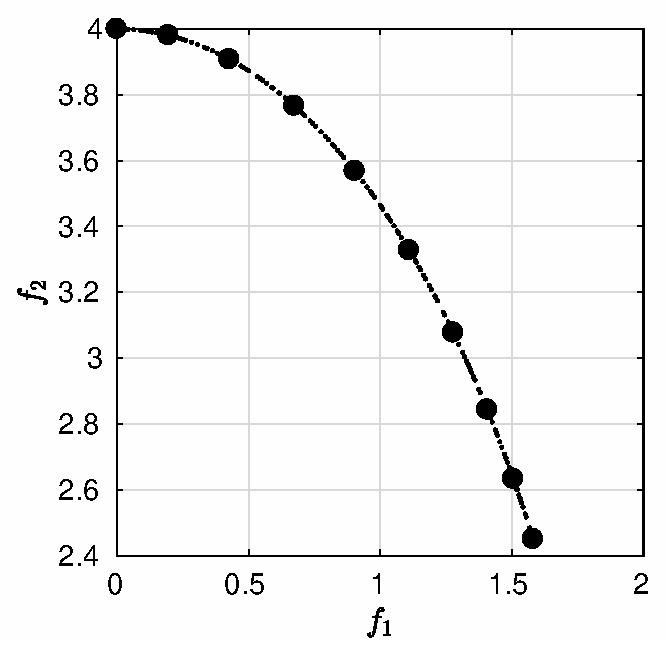
\includegraphics[width=0.3\textwidth]{figures/P1_PF.eps}
\label{fig:reference_sets_p1_PF}
}
\subfigure[P2: PF]{
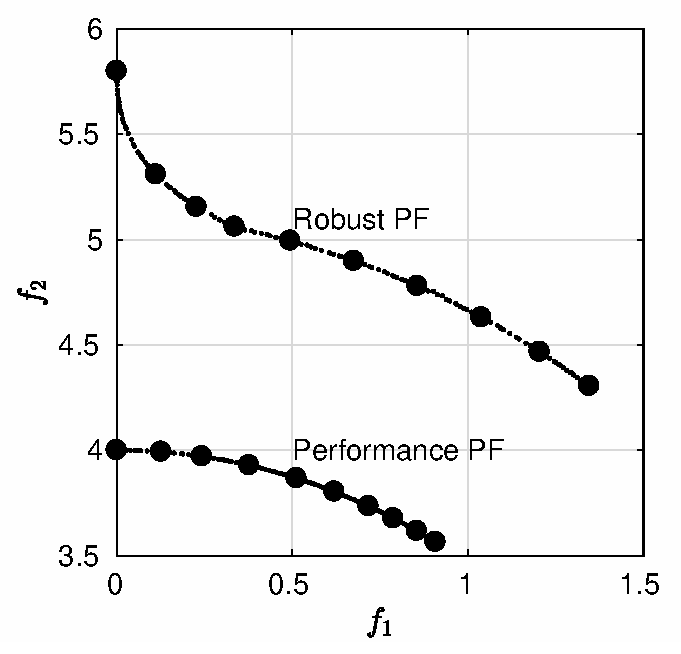
\includegraphics[width=0.3\textwidth]{figures/P2_PF.eps}
\label{fig:reference_sets_p2_PF}
}
\subfigure[P2: Decision vectors]{
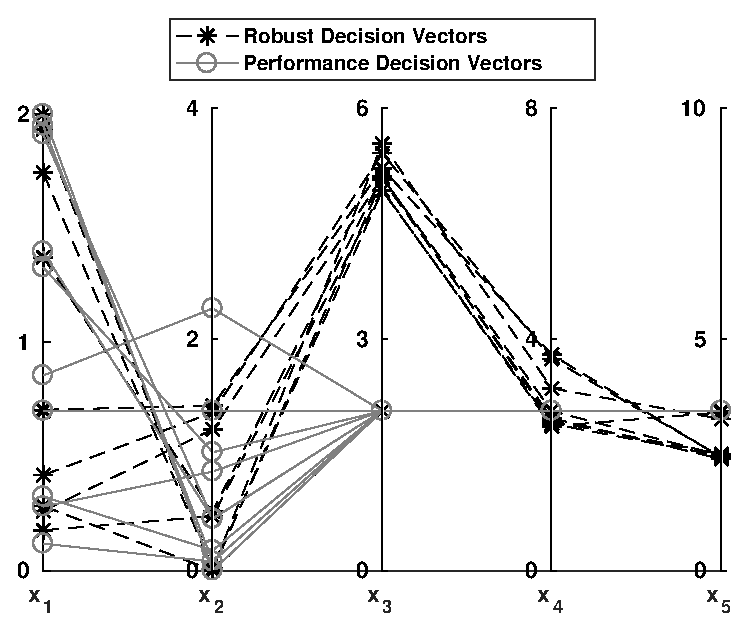
\includegraphics[width=0.32\textwidth]{figures/P2_PS.eps}
\label{fig:reference_sets_p2_PS}
}
\caption{Performance set for P1, and robust and performance sets for P2.}
\label{fig:reference_sets}
\end{figure}


\section{Experiment: Comparison of ParEGO and sParEGO}\label{sec:results}

\subsection{Experimental Settings}

In both ParEGO and sParEGO algorithms the scalarisation function corresponds to the augmented Tchebycheff and the simplex lattice approach is used for the generation of weight vectors, both these approaches have been taken from~\cite{Knowles2006ParEGO}. The weight vectors are modified by Generalised Decomposition approach~\cite{giagkiozis2014generalized} to provide a better estimate on the PF and we refer to them as reference direction vectors. The parameter settings for both algorithms are as follows: $n_{init} = 10$, $n_d = 10$, $n_{max} = 50$, and the optimization budget is set to 1000 function evaluations. For sParEGO the confidence level ($c$) is set to 90\%. Inverted Generalisation Distance (IGD)~\cite{bib:generational_distance} is used to measure the quality of the obtained sets by the optimizers. The 10 solutions that are marked with a filled circle in Figure~\ref{fig:reference_sets} are used as the reference sets for IGD, and these solutions correspond to the best trade-offs for the chosen direction vectors.


\subsection{Results and Observations}

This section presents the experimental results for P1 and P2 problems. The results shown in Figure~\ref{fig:algorithms_comparison} provide both a visual and a analytical assessment of the quality of the solutions obtained by the optimizers in terms of their convergence to and diversity across the PF. The objective vectors for P2 have been determined by evaluating 100 times each decision vector, obtained at the end of the optimization run, and the robust performance of each objective is equal to the 90\% percentile of its own marginal distribution. The performance of the objective vectors for P1 is equal to their (original) nominal performance since the problem does not contain uncertainty.

For P1, ParEGO approximation to the performance PF is better than sParEGO as shown in Figures~\ref{fig:P1_PF_comparison-a} and~\ref{fig:P1_PF_comparison-b}. ParEGO chosen solutions are not fully on the PF, but it is expected for its convergence to improve with more function evaluations since the trend shown in Figure~\ref{fig:P1_PF_comparison-b} indicates a declining IGD value. The same trend is captured for sParEGO, despite the fact that its convergence is worse than ParEGO. This indicates that the multi-modality in P1, close to the vinicity of the PF, is interpreted by sParEGO as a region of high uncertainty. The robust performance of the solutions in this region is captured as being poor by the statistical inferences made by sParEGO. Hence, most sParEGO solutions are just outside the region where the magnitude of the hill sizes of the multi-modality is considered to be higher. Nevertheless, it is expected for sParEGO to improve its convergence to the PF with more function evaluations, since the statistical assessment made about the true robust performance of the solutions that are on the PF is also expected to improve.

For P2, sParEGO approximation to the robust PF is better than ParEGO as shown in Figures~\ref{fig:P2_PF_comparison-a} and~\ref{fig:P2_PF_comparison-b}. The convergence of ParEGO deteriorates along the optimization run as shown in Figure~\ref{fig:P2_PF_comparison-b}, while the convergence of sParEGO improves. This indicates that the selection criterion used by ParEGO that promotes solutions with a better nominal performance, leads to a deteriorisation in the convergence towards the true robust solutions. On the other hand, the uncertainty quantification approach used by sParEGO that is used to estimate the true robustness of the solutions, is found to be a better approach in dealing with the task of finding the robust PF, for a given confidence level.

\begin{figure}
\centering
\subfigure[P1: Single run]{
 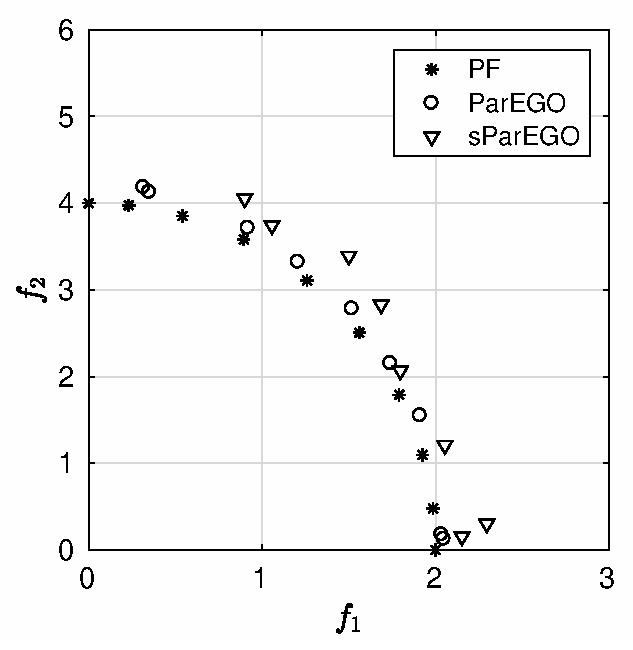
\includegraphics[width=0.4\textwidth]{figures/P1_PF_ParEGO_Vs_sParEGO.eps}
 \label{fig:P1_PF_comparison-a}
}
\hspace{1cm}
\subfigure[P2: Single run]{
 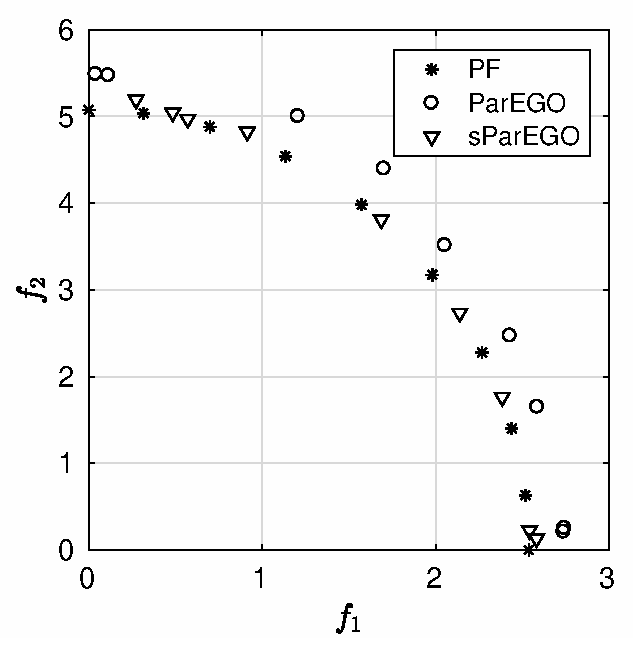
\includegraphics[width=0.4\textwidth]{figures/P2_PF_ParEGO_Vs_sParEGO.eps}
 \label{fig:P2_PF_comparison-a}
}
\\
\subfigure[P1: IGD]{
 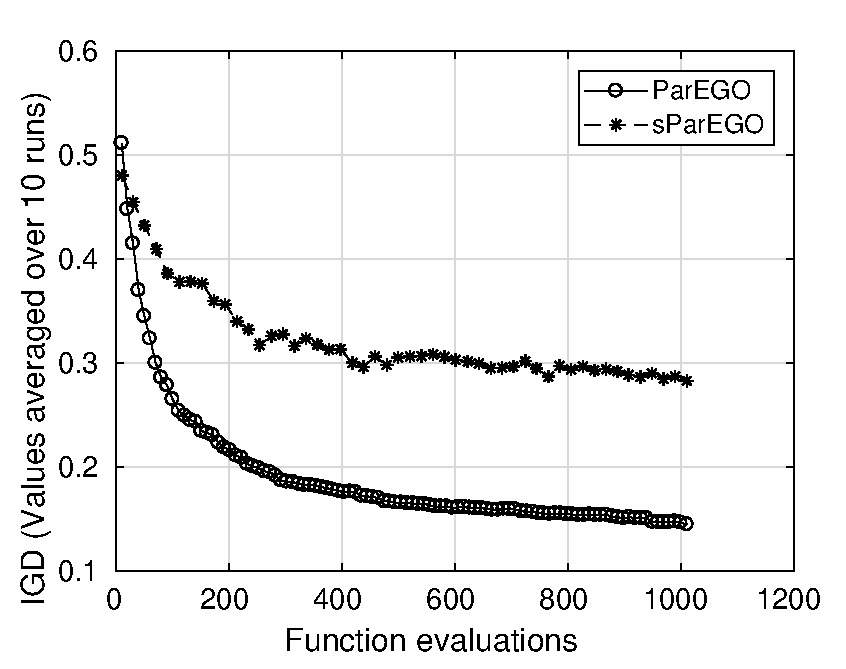
\includegraphics[width=0.4\textwidth]{figures/P1_IGD.eps}
 \label{fig:P1_PF_comparison-b}
}
\hspace{1cm}
\subfigure[P2: IGD]{
 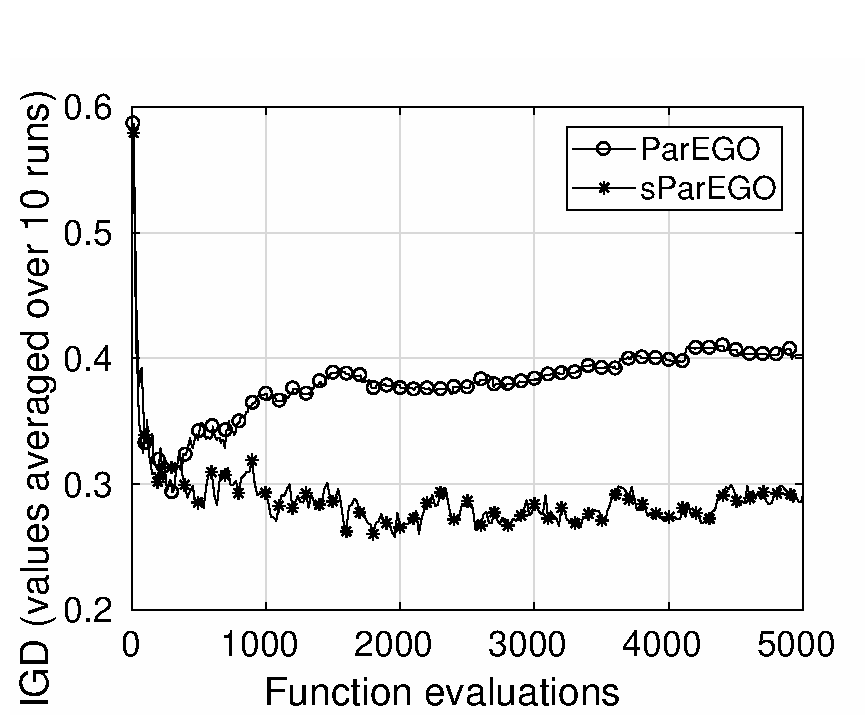
\includegraphics[width=0.4\textwidth]{figures/P2_IGD.eps}
 \label{fig:P2_PF_comparison-b}
}
\caption{Comparison of ParEGO and sParEGO for P1 and P2.}
\label{fig:algorithms_comparison}
\end{figure}

\section{Conclusion}\label{sec:conclusion}

This paper has proposed a new multi-objective optimization algorithm -- sParEGO -- for expensive uncertain MOPs. The comparative analysis with the existing algorithm ParEGO showed that sParEGO can offer superior performance in approximating a robust PF, but does not perform so well for problems with a highly non-smooth landscape. The latter finding is due to the assumption made by sParEGO that the stochastic performance of neighbouring solutions is similar. Further benchmarking of sParEGO is now needed to confirm its capabilities across a wider set of problem instances.
\vspace{2mm}

\textbf{Acknowledgements: }This work was supported by Jaguar Land Rover and the UK-EPSRC grant EP/L025760/1 as part of the jointly funded Programme for Simulation Innovation.

\small{
\bibliographystyle{splncs}
\bibliography{sparegoReferences}
}
\end{document}
